\documentclass[unicode, notheorems]{beamer}

\mode<presentation>
{
	\usetheme[numbers, totalnumbers, minimal]{Statmod}
	\setbeamercovered{transparent}
	\setbeamertemplate{caption}[numbered]
	\setbeamertemplate{enumerate item}[default]
	\setbeamertemplate{itemize item}[circle]
}

\usepackage[T2A]{fontenc}
\usepackage[utf8]{inputenc}
\usepackage[russian]{babel}
\usepackage{amsthm}
\usepackage{graphicx}
\usepackage{subfig}
\usepackage{bm}

\DeclareMathOperator{\E}{\mathbb{E}}
\DeclareMathOperator{\Prb}{\mathbb{P}}
\DeclareMathOperator*{\argmax}{arg\,max\ }

\title[Оценивание расстояния на графах де Брёйна]{Задачи оценивания геномного расстояния на графах де Брёйна}

\author[Константинов А. В., гр. 15.Б04-мм]{Константинов Антон Владимирович, гр. 15.Б04-мм}
\institute[СПбГУ]{
	\small
	Санкт-Петербургский государственный университет \\
	Прикладная математика и информатика \\
	Вычислительная стохастика и статистические модели \\
	\vspace{0.4cm}
	Научный руководитель: к.ф.-м.н., доцент Коробейников~А. И. \\
	Рецензент: м.н.с. Шлемов~А. Ю.
	\vspace{0.3cm}
}
\date{
	Санкт-Петербург\\
	2019
}

\begin{document}

\begin{frame}
	\titlepage
\end{frame}

\begin{frame}{Основные понятия, связанные с геномом}
	\begin{block}{}
	\begin{itemize}
		\item \textbf{Геномом} будем называть строку $\mathcal{S}$ над четырёхбуквенным алфавитом $\{A, T, G, C\}$.
		\item \textbf{Рид} (или \textbf{прочтение}) --- короткая подстрока $\mathcal{S}$.
		\item \textbf{$k$-мер} --- подстрока $\mathcal{S}$, имеющая длину $k$.
		\item \textbf{Спектр $k$-меров} --- множество всех $k$-меров, встречающихся в $\mathcal{S}$.
	\end{itemize}
\end{block}
\end{frame}

\begin{frame}{Задача сборки генома}
	Рассмотрим некоторый геном $\mathcal{S}$ и предположим, что имеется набор его  ридов. Обозначим его через $\mathfrak{R}$ и будем называть \textbf{библиотекой ридов} для $\mathcal{S}$.\\
	\vspace{0.5cm}
	\textbf{Задача сборки генома}: \\
	\vspace{0.1cm}
	По набору строк $\mathfrak{R}$ восстановить как можно более длинные \textbf{контиги} --- непрерывные подстроки исходной строки $\mathcal{S}$ (в идеале всю строку целиком).
\end{frame}

\begin{frame}{Граф де Брёйна}
	\textbf{Граф де Брёйна строки $\mathcal{S}$}:

	\begin{enumerate}
		\item В качестве вершин графа берётся спектр $k$-меров строки $\mathcal{S}$.
		\item Для каждого $(k+1)$-мера, содержащегося в $\mathcal{S}$, в граф добавляется ребро $v_1 \to v_2$, где $v_1$ и $v_2$ --- его префикс и суффикс длины $k$ соответственно.
		\item Количество таких рёбер равно количеству вхождений соответствующего $(k+1)$-мера в геном. 
	\end{enumerate}
	\vspace{0.2cm}
	\textbf{Замечание}: На практике вместо кратных рёбер обычно используют взвешенные, а однозначно продолжимые рёбра склеивают вместе.
\end{frame}

\begin{frame}{Свойства графа де Брёйна}
	\begin{block}{}
		\textbf{Эйлеров путь} в мультиграфе --- это путь, проходящий по каждому ребру мультиграфа ровно столько раз, какова его кратность.
	\end{block}
	\vspace{0.2cm}
	Пусть $G$ --- граф де Брёйна строки $\mathcal{S}$. Тогда
	\begin{enumerate}
		\item В этом графе \textbf{существует} соответствующий исходной строке $\mathcal{S}$ эйлеров путь. Будем называть этот путь \textbf{геномным}.
		\item Если в графе всего один эйлеров путь, то мы получаем возможность однозначно восстановить исходную строку.
	\end{enumerate}
\end{frame}

\begin{frame}{Сборка при помощи графа де Брёйна}
	Итак, есть библиотека ридов $\mathfrak{R}$.\\
	\vspace{0.2cm}

	\textbf{Проблема}: для построения графа де Брёйна требуется знать \textbf{все} $k+1$-меры \textbf{неизвестной} строки $\mathcal{S}$.\\
	\vspace{0.4cm}
	\textbf{Решение}: необходимо наложить на библиотеку ридов $\mathfrak{R}$ дополнительные условия.\\
	\vspace{0.3cm}
	Предположим, что риды из $\mathfrak{R}$ содержат все $(k+1)$-меры, имеющиеся в $\mathcal{S}$ (т. н. \textit{модель плотных ридов}).\\
	\vspace{0.1cm}
	
	Тогда можно извлечь из $\mathfrak{R}$ спектр её $(k+1)$-меров и построить граф де Брёйна, используя их.
\end{frame}

\begin{frame}{Проблемы подхода}
	Плохое качество сборки может быть следствием
	\begin{enumerate}
		\item Ошибок в ридах (неточных прочтений),
		\item Нарушения предположения о плотности покрытия генома ридами,
		\item Особенностей структуры генома --- повторы последовательностей (имеющие длину больше $k$) в $\mathcal{S}$ приводят к неединственности эйлерова пути.
	\end{enumerate}
\end{frame}

\begin{frame}{Повторы}
	Предположим, что геном имеет вид $\mathbf{e_1 f e_2 \ldots g_1 f g_2}$, где $\mathbf{e}_i$, $\mathbf{g}_i$ и $\mathbf{f}$ --- некоторые строки.

	\begin{figure}
		\centering
		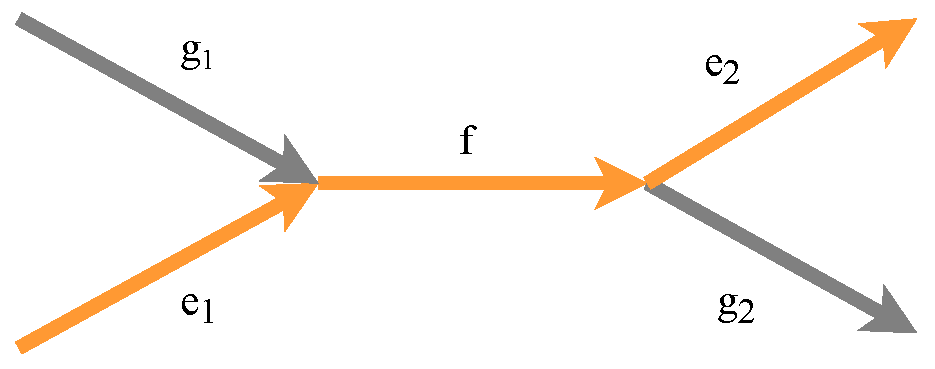
\includegraphics[scale=0.5]{img/repeat}
		\caption{Простой повтор в графе}
	\end{figure}

	Как должен проходить эйлеров путь,
	\begin{itemize}
		\item $\color{red} e_1 \to f \to e_2$ или $e_1 \to f \to g_2$?
		\item $\color{red} g_1 \to f \to g_2$ или $g_1 \to f \to e_2$?
	\end{itemize}
\end{frame}

\begin{frame}{Повторы}
	\begin{itemize}
		\item Следовательно, повторы жизненно необходимо каким-то образом разрешать.
		\item Для разрешения повторов в графе сборки обычно используются специальные структуры, несущие дополнительную информацию о связи между последовательностями на рёбрах графа.
		\item Одной из таких структур являются так называемые \textbf{парные риды}.
	\end{itemize}
\end{frame}

\begin{frame}{Вероятностная модель парных ридов}
%	\begin{block}{}
%		\begin{itemize}
%			\item \textbf{Фрагмент} --- подстрока $\mathcal{S}$, имеющая вид $\mathcal{S}[\xi, \xi+\eta]$, где $\xi$ --- случайная координата начала фрагмента, а $\eta$ --- случайная длина фрагмента (т. н. \textbf{длина вставки}).
%			\item \textbf{Парный рид} --- пара $(r_1, r_2)$, где $r_1$ --- префикс фрагмента (\textit{forward-рид}), $r_2$ --- его суффикс (\textit{reverse-рид}).
%		\end{itemize}
%	\end{block}
	
%	\begin{figure}
%		\centering
%		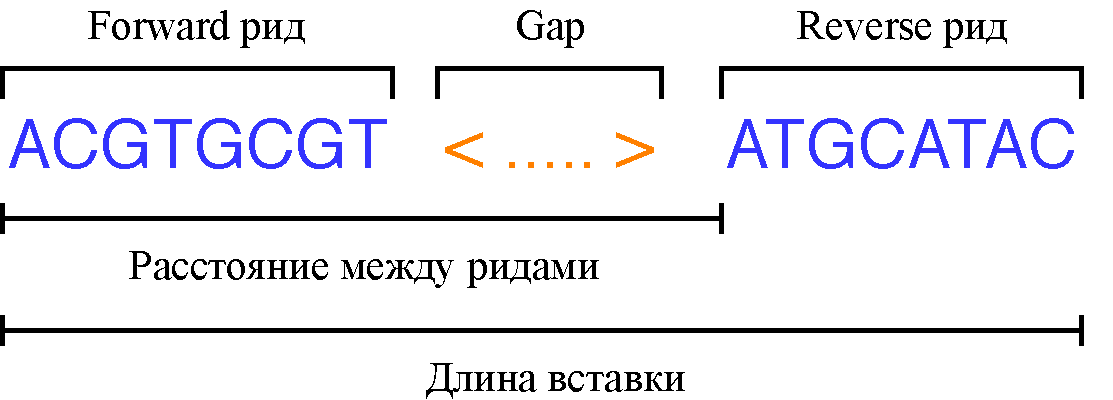
\includegraphics[scale=0.5]{img/paired-end-read}
%		\caption{Структура парного рида}
%	\end{figure}
	Пусть
	\begin{itemize}
		\item  $\xi$ --- дискретная случайная величина с носителем $\{ 1, \ldots, |\mathcal{S}|\}$, имеющая смысл координаты в геноме,
		\item $\eta$ --- независимая от $\xi$ неотрицательная целочисленная случайная величина (т. н. \textbf{длина вставки}),
		\item $\ell$ --- положительное целое число (\textbf{длина рида}).
	\end{itemize}
	\begin{block}{}
			\begin{enumerate}
				\item Фрагмент --- подстрока генома, имеющая вид $\mathcal{S}[\xi, \xi+\eta]$;
				\item Левый рид --- префикс длины $\ell$ фрагмента, т. е. подстрока  $\mathcal{S}[\xi, \xi+\ell]$;
				\item Правый рид --- суффикс длины $\ell$ фрагмента, т.е. подстрока $\mathcal{S}[\xi+\eta-\ell, \xi+\eta]$.
			\end{enumerate}
	\end{block}
\end{frame}

\begin{frame}{Разрешение повторов}
	\begin{figure}	
		\centering
%		\includegraphics[scale=0.45]{img/repeпat-resolution}
%		\caption{Простой повтор}t
	\end{figure} 

	\textbf{Графовое расстояние} между $r_1$ и $r_2$ вдоль $\mathbf{p} = (e_1, f, e_2)$: 
	\begin{equation*}
		d_{graph}(r_1, r_2) = d(e_1, e_2) - r_1^{(s)} + r_2^{(s)},
	\end{equation*}
	где $d(e_1, e_2) = |\mathbf{p}| - |e_2|$ --- расстояние между $e_1$ и $e_2$ вдоль $\mathbf{p}$, $r_i^{(s)}$ --- координата начала $r_i$ на $e_i$.
\end{frame}

\begin{frame}{Разрешение повторов}
	Предположим, что длины ридов и длина вставки известны точно.\\
	\vspace{0.3cm}
	В этом случае известно \textbf{геномное расстояние} между $r_1$ и $r_2$ (то есть расстояние между ними как подстроками генома):\\
	\begin{equation*}
		d_{genome}(r_1, r_2) = L - |r_2|,
	\end{equation*}
	где $L$ --- точное значение длины вставки.\\
	\vspace{0.3cm}
	Тогда если \[d_{graph}(r_1, r_2) \ne d_{genome}(r_1, r_2),\] то можно утверждать, что путь $\mathbf{p} = (e_1, f, e_2)$ не является частью геномного пути.
\end{frame}

\begin{frame}{Постановка задачи}
	\begin{figure}	
		\centering
		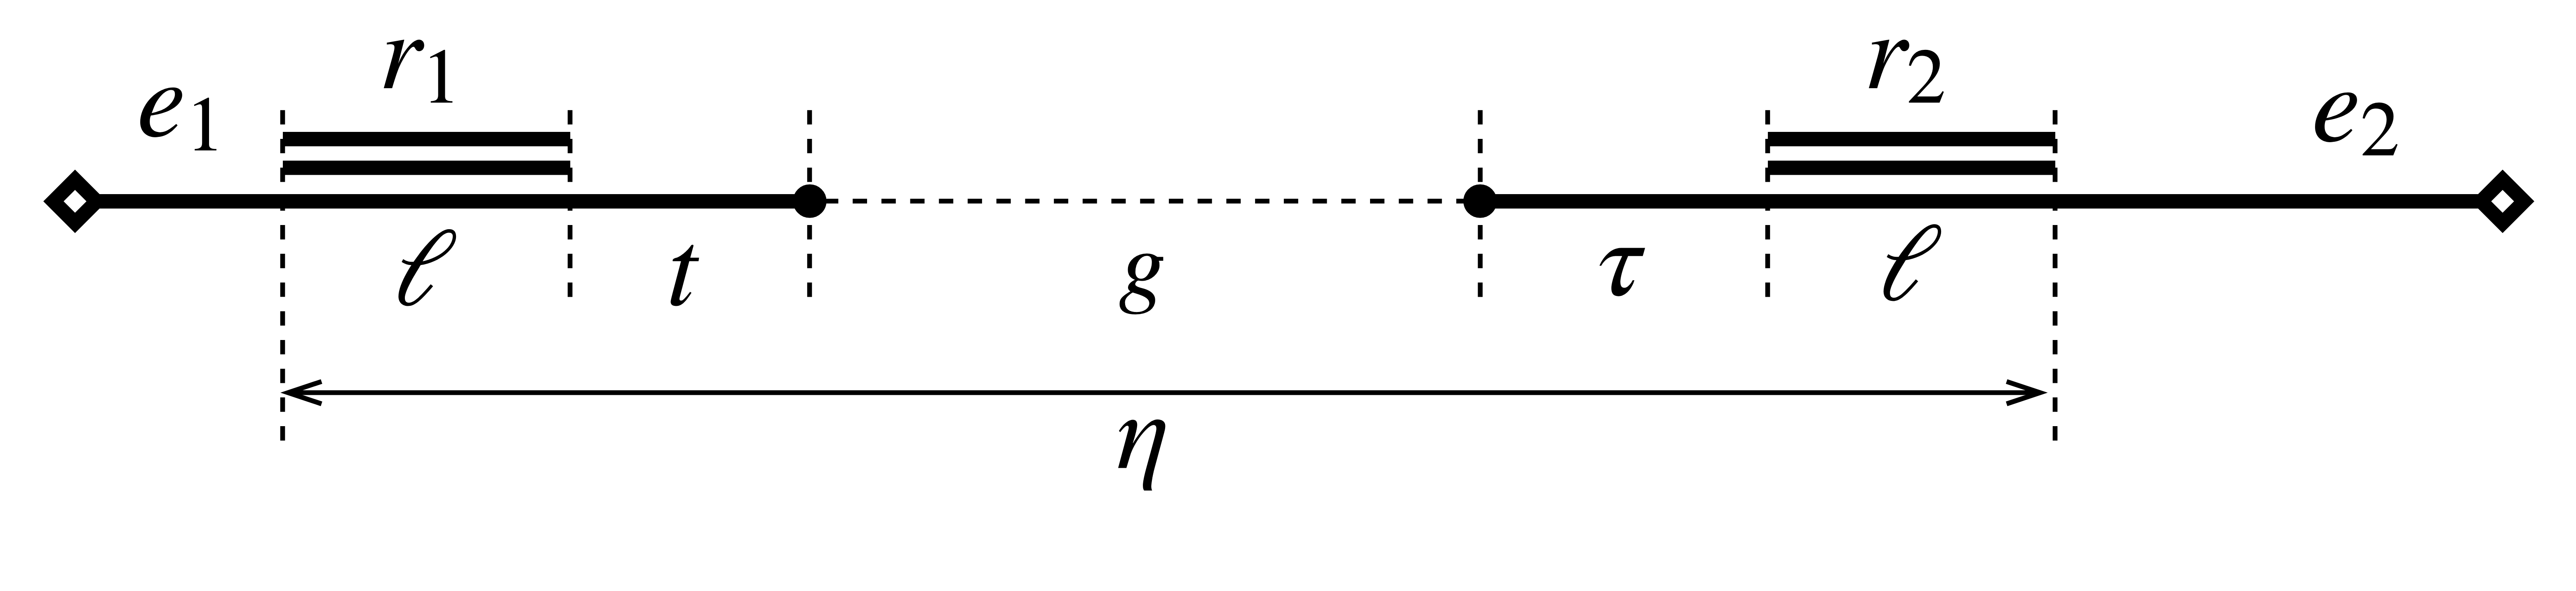
\includegraphics[scale=0.05]{img/alignment_shifted}
		\caption{Расположение ридов на рёбрах графа}
	\end{figure}

	Зафиксируем пару рёбер $e_1$, $e_2$. Пусть известны координаты ридов $r_i$ на рёбрах $e_i$. Введём обозначения: 
	\begin{enumerate}
		\item $g$ --- \textbf{гэп} между $e_1$ и $e_2$,
		\item $t$ --- расстояние от конца $r_1$ до конца $e_1$,
		\item $\tau$ --- координата начала $r_2$ на $e_2$.
	\end{enumerate}
\end{frame}

\begin{frame}{Постановка задачи}
	Рассмотрим формально выборку \[ \mathbb{T}^\prime = \Big( (t_1, \tau_1, g_1), \ldots, (t_n, \tau_n, g_n) \Big) \] из совместного распределения $t$, $\tau$ и $g$.\\
	\vspace{0.2cm}
	Будем считать, что рид $r_1$ приложен к ребру $e_1$.  Введём событие \[ A_{e_2}(r_2) = \{\text{рид } r_2 \text{ приложен к } e_2\}. \]
	\vspace{0.2cm}
	На самом деле, мы наблюдаем реализации только при условии $A_{e_2}$, а $g_i$ не наблюдаем вовсе.\\
	\vspace{0.2cm}
	Получаем набор реализаций
	\[ \mathbb{T} = \Big( (t_1, \tau_1), \ldots, (t_n, \tau_n) \Big). \]
\end{frame}
\begin{frame}{Постановка задачи}
	Пусть \[\mathbf{D}_{graph} = \{g^{(1)}, \ldots, g^{(k)}\}\] --- набор гэпов между рёбрами $e_1$ и $e_2$ в графе сборки, а
	$\mathbf{D}_{genome}$ --- набор гэпов между ними в геноме.\\
	\vspace{0.2cm}
	Положим \[ \mathbf{D} = \mathbf{D}_{genome} \cap \mathbf{D}_{graph}. \]
\end{frame}
\begin{frame}{Постановка задачи}
	Совместное распределение вектора $(t_i, \tau_i)$ зависит от $g_i$ как от параметра. При этом $t_i$, $\tau_i$ и $g_i$ связаны соотношением
	\begin{equation*}
		\tau_i = \eta_i - t_i - g_i - 2\ell,
	\end{equation*}
	где $g_i  \in \mathbf{D}$ --- один из графовых гэпов,  который одновременно является и геномным.\\
	\vspace{0.5cm}
	\textsc{Задача}: определить, какие из $g^{(i)} \in \mathbf{D}_{graph}$ являются геномными, при помощи выборки $\mathbb{T}$.
\end{frame}

%\begin{frame}{Априорная информация}
%	Кроме выборки $\mathbb{T}$ мы также располагаем и некоторой \textit{априорной} информацией --- набором \[\mathbb{D} = \{g^{(1)}, \ldots, g^{(k)}\}\] расстояний между рёбрами $e_1$ и $e_2$ в графе.\\
%	\vspace{0.2cm}
%	То есть мы можем ввести естественным образом \textit{априорное распределение} для $g$:
%	\begin{equation*}
%		g \sim \begin{pmatrix} g^{(1)} & \ldots & g^{(k)} \\ 1/k & \ldots & 1/k \end{pmatrix}.
%	\end{equation*}
%\end{frame}

\begin{frame}{Правдоподобие (одно наблюдение)}
	Здесь и далее в формулах для упрощения будем опускать условие $A_{e_2}$.
\begin{block}{Предложение}
	Пусть $\eta = \lfloor \tilde{\eta} \rfloor$, где $\tilde{\eta}$ имеет распределение $\mathrm{N}(\mu, \sigma^2)$ с известными средним $\mu$ и дисперсией $\sigma^2$.\\
	\vspace{0.2cm}
	Тогда
	\begin{equation*}
	\begin{gathered}
	p(g | \tau, t) =  \frac{q(\tau, g, t)}{\sum_{j=1}^k q(\tau, g^{(j)}, t)}	\,,
	\end{gathered}
	\end{equation*}
	где
	\begin{equation*}
	q(x, y, z)  = \frac{\Phi\big(x+y+z+2\ell+1\big) - \Phi\big(x+y+z+2\ell\big)}{1 - \Phi\big(y + z + 2\ell\big)}\,,
	\end{equation*}
	а $\Phi$ --- функция распределения закона $\mathrm{N}(\mu, \sigma^2)$.
\end{block}
\end{frame}

\begin{frame}{Переход к множественным наблюдениям}
	\begin{itemize}
		\item Пусть имеется библиотека парных ридов $\mathcal{R}$.
		\item На практике для каждого рида  $(r_1, r_2) \in \mathcal{R}$ реализуется собственный гэп $g^{(i)} \in \mathbf{D}_{genome}$ для некоторого $i$.
		\item Поэтому нельзя напрямую использовать статистический вывод по повторной независимой выборке из распределения $(\tau, t)$.
	\end{itemize}
\end{frame}

\begin{frame}{Модель}
	\begin{itemize}
		\item Формально $(\tau, t, g) \sim \mathcal{P}_{\tau, t, g}$\,, где на $g$ накладывается априорное распределение:
		\begin{equation*}
			g \sim  \begin{pmatrix} g^{(1)} & \ldots & g^{(k)} \\ 1/k & \ldots & 1/k \end{pmatrix}.
		\end{equation*}
		\item На практике $g$ --- скрытая переменная, распределение которой мы хотим оценить.
	\end{itemize}
%	Так как $i$ определяется исключительно эмпирическим распределением выборки $\mathbb{T}$, то можно считать, что
%	\begin{equation*}
%			i \sim \mathrm{U}(n).
%	\end{equation*}
\end{frame}

\begin{frame}{Апостериорное распределение (набор наблюдений)}
	\begin{block}{Предложение}
		В тех же условиях
		\begin{equation*}
			p(g | \mathbb{T}) = \frac{1}{n} \sum_{i = 1}^n \left[ \frac{q(\tau_i, g, t_i)}{\sum_{j=1}^k q(\tau_i, g^{(j)}, t_i)} \right]\,,
		\end{equation*}
		где
		\begin{equation*}
			q(x, y, z)  = \frac{\Phi\big(x+y+z+2\ell+1\big) - \Phi\big(x+y+z+2\ell\big)}{1 - \Phi\big(y + z + 2\ell\big)}\,,
		\end{equation*}
		а $\Phi$ --- функция распределения закона $\mathrm{N}(\mu, \sigma^2)$.
	\end{block}
\end{frame}

\begin{frame}{Моделирование}
	За основу были взяты первые 400 тысяч нуклеотидов генома \textit{E.coli}. При помощи пакета \textbf{art} были промоделированы парные риды с длиной вставки, имеющей распределение $\mathrm{N}(1000, 30)$.\\
	\vspace{0.3cm}
	По получившимся ридам при помощи геномного ассемблера \textbf{SPAdes} был построен граф де Брёйна.\\
	\vspace{0.3cm}
	Для выравнивания рёбер получившегося графа на исходный геном и выравнивания ридов на рёбра использовался пакет \textbf{bwa}.
\end{frame}

\begin{frame}{Пример апостериорных вероятностей}
	\begin{figure}%
		\centering
		\subfloat[Граф]{{\includegraphics[width=0.4\linewidth, scale=0.4]{img/graph_183748_183600} }}%
		\qquad
		\subfloat[Распределение]{{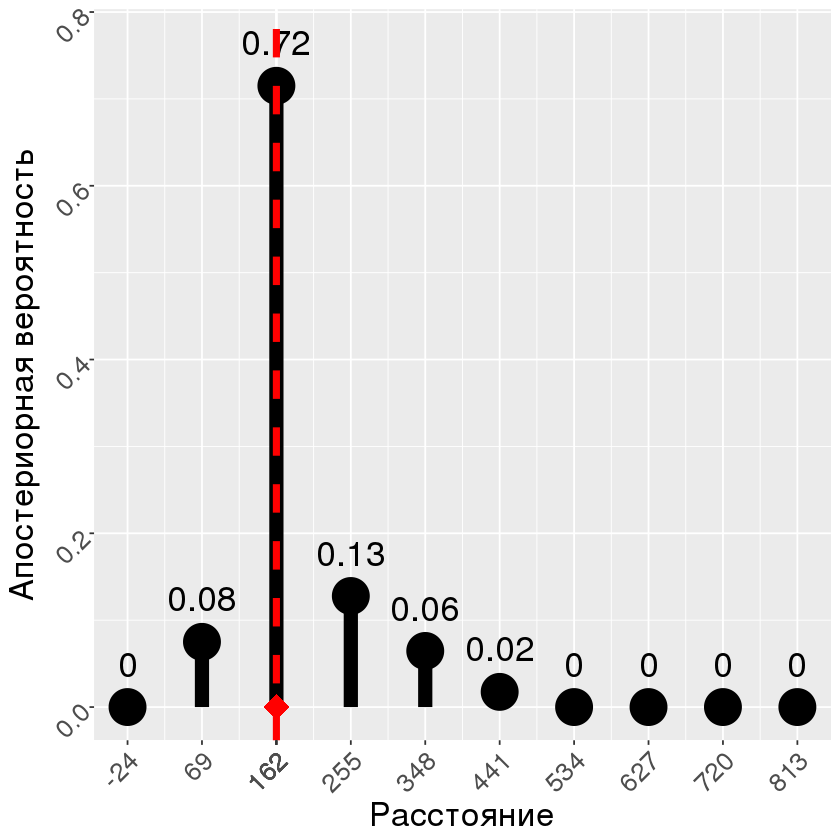
\includegraphics[width=0.5\linewidth]{img/183600_183748} }}%
	\end{figure}
\end{frame}

%\begin{frame}{Прямое моделирование}
%	Пусть $\mu = 1000$, $\sigma = 30$, $\ell = 100$. В качестве априорного распределения $g$ выберем равномерное дискретное со значениями из $\{100,  200, \ldots, 800\}$.\\
%	\vspace{0.2cm}
%	\begin{enumerate}
%		\item Промоделируем выборку с $g$ из априорного распределения,
%		\item Промоделируем выборку с $g$ из распределения, отличного от априорного.
%	\end{enumerate}
%	В обоих случаях сравним получаемое условное распределение с вычисленным теоретически.
%\end{frame}

%\begin{frame}{Моделирование (прямое)}
%	Моделируем $g$ из априорного распределения.
%	\begin{figure}
%			\centering
%			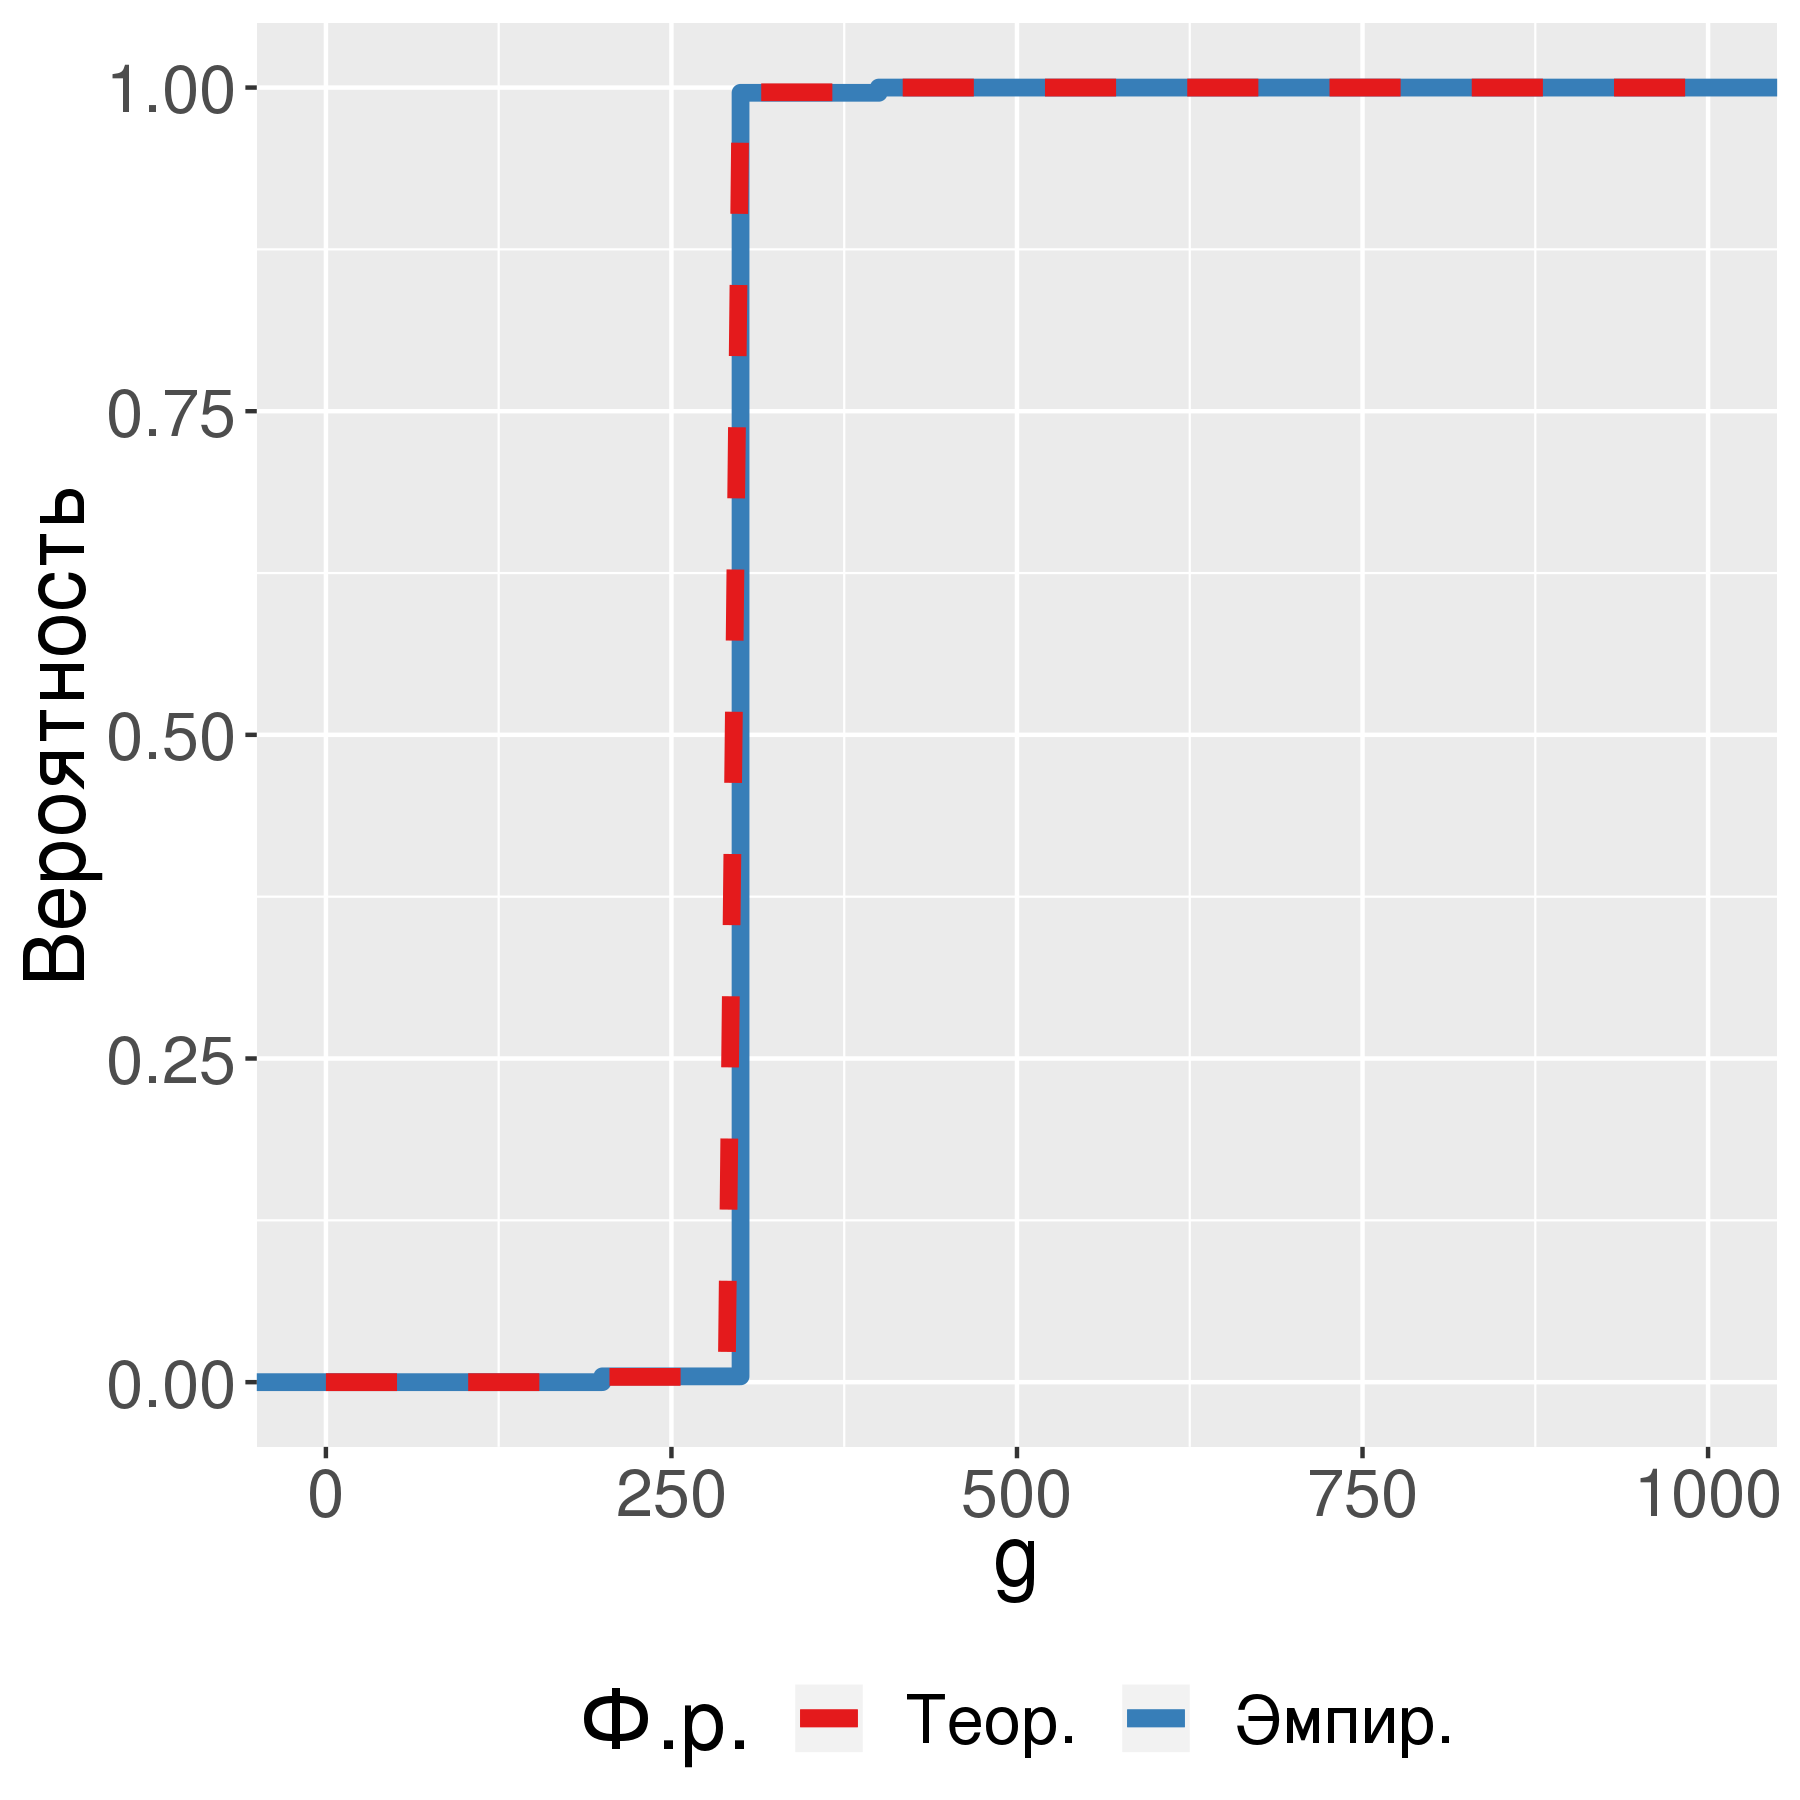
\includegraphics[scale=0.45]{img/cdf1}
%	\end{figure}
%\end{frame}

%\begin{frame}{Моделирование (прямое)}
%Теперь пусть $g$ всегда равно $550$, а априорное распределение по-прежнему сосредоточено на $\{100, \ldots, 800\}$.
%\begin{figure}
%	\centering
%	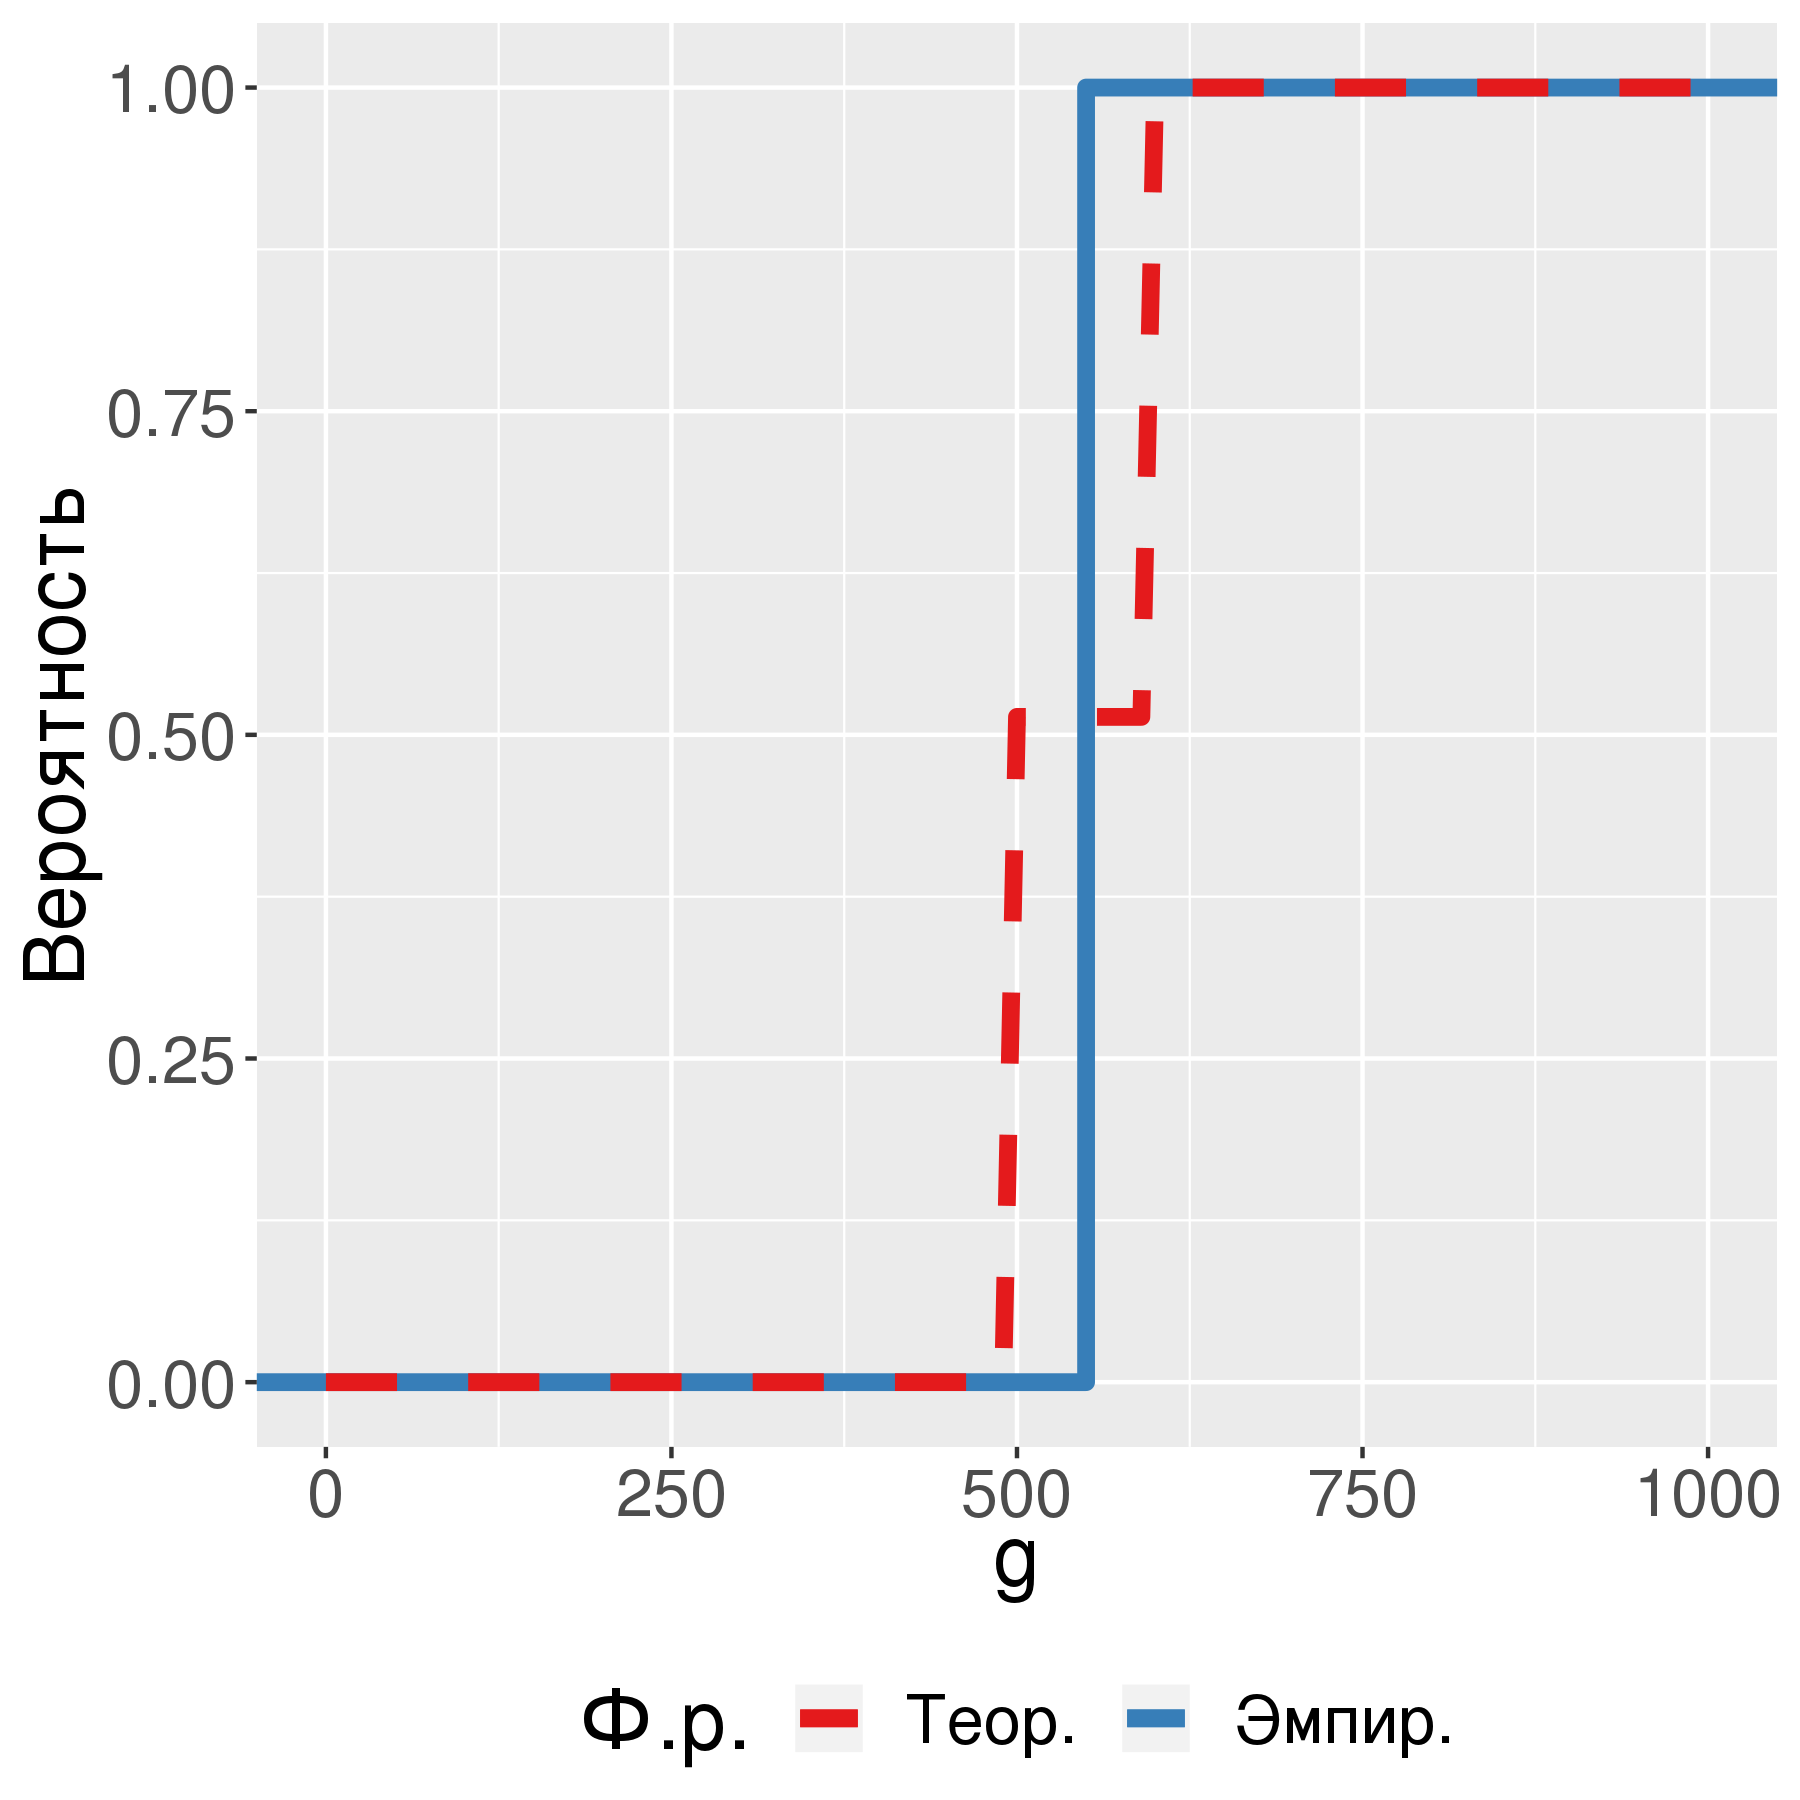
\includegraphics[scale=0.45]{img/cdf2}
%	\caption{$g$ моделируется из априорного распределения}
%\end{figure}
%\end{frame}

%\begin{frame}{Дальнейшие планы}
%Проверить полноценно на реальном геноме --- с построением графа, выравниванием ридов на рёбер:
%\begin{enumerate}
%	\item На симулированных ридах,
%	\item На реальных ридах.
%\end{enumerate}
%\end{frame}

%\begin{frame}{Выборка расстояний между рёбрами}
%	\begin{itemize}
%		\item Предположим, имеется парный рид $(r_1,r_2)$ и координаты $r_1$ и $r_2$ на рёбрах $e_1$ и $e_2$ соответственно.
%		\item  Расстояние между рёбрами:
%		\begin{equation*}
%			d(r_1,r_2) = \eta - |r_2| + r_1^{(s)} - r_2^{(s)},
%		\end{equation*}
%		где $r_i^{(s)}$ --- координаты начала $r_i$ на $e_i$, а $\eta$ --- длина вставки.
%	\end{itemize}
%	\begin{block}{}
%		$\mathbb{X}_{e_1,e_2} = \left\{ d(r_1,r_2)\ |\ r_i \text{ является подстрокой } e_i \right\}$ --- выборка расстояний между $e_1$ и $e_2$.
%	\end{block}
%\end{frame}

%\begin{frame}{Постановка задачи}
%	Зафиксируем $e_1$ и $e_2$.\\
%	\begin{itemize}
%		\item Пусть $\mathcal{P} = \mathcal{P}_{e_1, e_2}$ ---  распределение расстояний между $e_1$ и $e_2$.
%		\item Так как оба ребра могут встречаться в геноме несколько раз, то и расстояний между ними может быть несколько.
%	\end{itemize}
%	\vspace{0.2cm}
%	\textbf{Входные данные}: 
%	\begin{enumerate}
%		\item $\mathbb{X} = \mathbb{X}_{e_1, e_2}$ --- выборка расстояний между $e_1$ и $e_2$,
%		\item Графовые пути между $e_1$ и $e_2$.
%	\end{enumerate}
%	\textbf{Задача}: построить модель, которая по выборке $\mathbb{X}$ позволит оценивать геномные расстояния между рёбрами $e_1$ и $e_2$, а также отличать потенциально геномные пути между ними от негеномных.
%\end{frame}

%\begin{frame}{Существующее решение}
%	В геномном сборщике \textbf{SPAdes} реализована следующая процедура оценки расстояний:
%	\begin{enumerate}
%		\item Строится упорядоченный по возрастанию набор графовых расстояний между $e_1$ и $e_2$.
%		\item Выбрасываются все графовые расстояния, которые отстоят от границ выборки $\mathbb{X}$ более чем на $\alpha \sigma_{\xi}$, где $\alpha$ --- настраиваемый коэффициент.
%		\item Для каждого элемента выборки находится ближайшее графовое расстояние, и к его весу прибавляется $1$ (если их два, то добавляется по $1/2$ каждому).
%		\item Далее над получившимся взвешенным набором расстояний производится иерархическая кластеризация. \item Оценка расстояний --- центроиды кластеров.
%	\end{enumerate}
%\end{frame}

%\begin{frame}{Существующее решение}
%	\begin{itemize}
	%	\item Иногда происходят ошибки сборки --- на гистограмме наблюдаемых расстояний наблюдается <<пик>>, но соответствующего ему пути в графе нет. Информация об этом полностью теряется.
	%	\item Хотелось бы получить модель, которая бы позволила избежать потери этой информации.
%	\end{itemize}
%\end{frame}

%\begin{frame}{Модель смеси распределений}
%	\begin{equation*}
	%	\mathcal{P} = \sum_{i=1}^n \pi_i \mathcal{P}^{(i)},
%	\end{equation*}
%	где
%	\begin{enumerate}
	%	\item $n$ --- количество геномных путей из $e_1$ в $e_2$;
	%	\item $\pi_i$ --- веса, то есть $\pi_i > 0$ и $\sum_{i=1}^n \pi_i = 1$;
	%	\item $\mathcal{P}^{(i)}$ --- абсолютно непрерывное распределение, математическое ожидание которого равно одному из геномных %расстояний.
%	\end{enumerate}
%\end{frame}

%\begin{frame}{Модель смеси нормальных распределений}
%	Предположим, что $\mathcal{P}^{(i)} = \mathrm{N}(d_i, \sigma_i^2)$, где $d_i$ --- длина одного из геномных путей.
%	Тогда плотность распределения расстояния имеет вид
%	\begin{equation*}
	%	\varphi(t) = \sum_{i=1}^n \pi_i \varphi_{d_i,\sigma_i^2}(t),
%	\end{equation*}
%	\vspace{0.3cm}
%	где $\varphi_{\mu,\sigma^2}$ --- плотность распределения $\mathrm{N}(\mu, \sigma^2)$.
%	\begin{itemize}
	%	\item Модель содержит $3n-1$ параметр: $\pi_j$ и $d_i$, $\sigma_i^2$ ($i \in 1:n$, $j\in 1:n-1$).
	%	\item Параметры можно оценить по выборке $\mathbb{X}$.
%	\end{itemize}
%\end{frame}

%\begin{frame}{Оценка параметров}
%	Для оценки параметров модели воспользуемся методом максимального правдоподобия. Обозначим
%	\begin{gather*}
%	\bm\pi = (\pi_1, \ldots, \pi_{n-1}),\ \bm d = (d_1, \ldots, d_n),\ \bm v = (\sigma_1^2, \ldots, \sigma_n^2),\\
%	\bm\theta = (\bm\pi, \bm d, \bm v),\\
%	\mathbb{X} = (X_1, \ldots, X_N).
%	\end{gather*}
%	Логарифмическая функция правдоподобия для нашей модели имеет вид
%	\begin{equation*}
%	\ell(\bm\theta; \mathbb{X}) = \sum_{j=1}^N \log \left( \sum_{i=1}^n \pi_i \varphi_{d_i,\sigma_i^2} (X_j)  \right).
%	\end{equation*}
%	Оптимизировать эту конструкцию по $\bm\theta$ напрямую не представляется возможным аналитически и весьма сложно численно.
%\end{frame}

%\begin{frame}{EM-алгоритм для нормальной смеси}
%	Рассмотрим  <<скрытые>> случайные векторы $\bm \Delta_j$ ($j \in 1:N$):
%	\begin{gather*}
	%	\bm \Delta_j^{(i)} = \left[ X_j \text{ порождено $i$-й компонентой смеси} \right].
%	\end{gather*}
	
%	\textbf{Шаг E(xpectation)} Считая $\bm\theta$ известным и равным $\bm\theta_0$, вычислим
%	\begin{equation*}
	%	\bm\gamma_j = \E \left[\bm\Delta_j | \bm\theta_0, \mathbb{X} \right], i \in 1:N.
%	\end{equation*}
	
%	\textbf{Шаг M(aximization)} Используя $\bm\Gamma = (\bm\gamma_1, \ldots, \bm\gamma_N)$, вычислим оценку $\bm\theta$:
%	\begin{gather*}
%		\hat{\pi}_i = \sum_{j=1}^N \gamma_i^{(j)},\quad
	%	(\hat{\bm d}, \hat{\bm v}) = \argmax_{\bm d, \bm v} \ell(\hat{\bm\pi}, \bm d, \bm v; \mathbb{X}),\\
	%	\hat{\bm \theta} = (\hat{\bm\pi}, \hat{\bm d}, \hat{\bm v}).
%	\end{gather*}
%	 Пары \textbf{E}- и \textbf{M}-шагов повторяются до сходимости.
%\end{frame}

%\begin{frame}{Программная реализация}
%	\textbf{Пакет mclust} реализует множество инструментов для работы со смесями нормальных распределений.
%	\begin{itemize}
	%	\item Оценка параметров производится при помощи EM-алгоритма.
	%	\item Оптимальное число компонент смеси выбирается автоматически на основании \textit{байесовского информационного критерия (BIC)}:
	%	\begin{equation*}
	%		BIC = k \log N - 2 \log L^*,
	%	\end{equation*}
	%	где $k = 3n-1$ --- число оцениваемых параметров, $n$ --- количество компонент смеси, $N$ --- объем выборки, $L^*$ --- максимальное значение правдоподобия.
%	\end{itemize}
%\end{frame}

%\begin{frame}{Решающее правило}
%	Оценки расстояний между рёбрами графа получены. Теперь требуется определить правило, по которому мы сможем отличать геномные пути от негеномных. \\
%	\vspace{0.2cm}
%	Воспользуемся для этого классификацией на основе полученной нами модели. \\
%	\vspace{0.3cm}
%	\textbf{Решающее правило}\\
%	Будем классифицировать путь длины $d$ как геномный, если найдётся такое $i$, что
%	\begin{equation*}
%	d_i - \sigma_i \le d \le d_i + \sigma_i,
%	\end{equation*}
%	где $d_i$ и $\sigma_i$ --- оценки параметров смеси, полученные при помощи EM-алгоритма.
%\end{frame}

%\begin{frame}{Данные и результаты классификации}
%	\textbf{Данные}: геном \textit{E. coli} и библиотека парных ридов с длиной вставки $298 \pm 17$. \\
%	\textbf{Объём генома}: 4.7 Mbp.\\
%	\vspace{0.3cm}
	
%	\textbf{Качество классификации}:\\
%	\textit{Accuracy} (доля правильно классифицированных): 0.59, \\
%	\textit{Точность} (доля правильно классифицированных как негеномные): 0.75, \\
%	\textit{Полнота} (доля выявленных негеномных): 0.71.\\
%	\vspace{0.3cm}
%	\textbf{Вывод}: классификатору удаётся довольно удачно отсеивать негеномные пути, хотя качество \textit{в целом} --- не лучшее.
%\end{frame}

%\begin{frame}{Данные и результаты классификации}
%	Классификация здесь оказывается плохой сразу по нескольким причинам:
%	\begin{itemize}
	%	\item Несбалансированность классов --- негеномных путей значительно больше, чем геномных.
	%	\item Большое количество ложно-отрицательных срабатываний объясняется тем, что многие истинные расстояния на самом деле \textbf{не могут} наблюдаться из-за недостаточной длины вставки.
%	\end{itemize}
%\end{frame}

%\begin{frame}{Дальнейшие планы}
%	\begin{itemize}
	%	\item Сравнить подход, реализованный в \textbf{SPAdes}, с \textbf{GMM} на уровне оценённых расстояний. Это осложняется тем, что как правило эти подходы выдают <<разное>> количество расстояний.
	%	\item Попытаться улучшить текущую модель.
	%	\item Опробовать иные модели.
%	\end{itemize}
%\end{frame}

\end{document}
